% Template for ICIP-2026 paper; to be used with:
%          spconf.sty  - ICASSP/ICIP LaTeX style file, and
%          IEEEbib.bst - IEEE bibliography style file.
% --------------------------------------------------------------------------
\documentclass{article}
\usepackage{spconf,amsmath,graphicx}
\usepackage{graphicx}%
\usepackage{multirow}%
\usepackage{amsmath,amssymb,amsfonts}%
\usepackage{amsthm}%
\usepackage{mathrsfs}%
\usepackage[title]{appendix}%
\usepackage{xcolor}%
\usepackage{textcomp}%
\usepackage{manyfoot}%
\usepackage{booktabs}%
\usepackage{algorithm}%
\usepackage{algorithmicx}%
\usepackage{algpseudocode}%
\usepackage{listings}%
% Example definitions.
% --------------------
\def\x{{\mathbf x}}
\def\L{{\cal L}}

% Title.
% ------
% \title{Learning from Imperfect Pseudo-Labels via Fine-Grained Grouping and Geometric Upsampling for Semi-Supervised 3D Object Detection}
\title{Towards Robust Multimodal Perception: Enhancing Sparse Geometric Representations for Semi-Supervised 3D Detection}
% \title{Semi-Supervised Learning via Fine-Grained Grouping and Geometric Upsampling for Semi-Supervised 3D Object Detection}
% \name{
% Shaojing Song$^{1}$ \quad
% Xinjian Li$^{2}$ \quad
% Fan Wu$^{3}$\quad
% Yumei Gong$^{1}$\sthanks{Corresponding author.}  \quad %
% Zhiqing Miao$^{4}$  \quad \\
% Xianxun Zhu$^{5,6,7}$  \quad
% Hui Chen$^{7}$  \quad
% Zhangkai Wu$^{7}$  \quad
% }
\name{
\textit{Shaojing Song}$^{1}$ \quad
\textit{Xinjian Li}$^{2}$ \quad
\textit{Fan Wu}$^{3}$\quad
\textit{Yumei Gong}$^{1}$\sthanks{Corresponding author.}  \quad %
\textit{Zhiqing Miao}$^{4}$  \quad \\
\textit{Xianxun Zhu}$^{5,6,7}$  \quad
\textit{Hui Chen}$^{7}$  \quad
\textit{Zhangkai Wu}$^{7}$  \quad
}
\address{
$^{1}$ School of Computer and Information Engineering, Shanghai Polytechnic University\\
$^{2}$ School of Intelligent Manufacturing and Control Engineering, Shanghai Polytechnic University\\
$^{3}$ School of Transportation, Southeast University\\
$^{4}$ School of Information and Electronic Engineering, East China Normal University\\
$^{5}$ School of Communication and Information Engineering, Shanghai University\\
$^{6}$ College of Computing and Data Science, Nanyang Technological University\\
$^{7}$ School of Computing, Macquarie University
}
\begin{document}
\maketitle
\begin{abstract}
% Fully supervised 3D object detection relies on large-scale point cloud annotations, which are costly and difficult to acquire in real-world. Semi-supervised learning (SSL) reduces annotation demand by leveraging unlabeled data, yet existing SSL-based methods often employ fixed confidence thresholds for pseudo-label selection, leading to information loss and unreliable supervision under sparse and misaligned point cloud observations. This paper proposes a semi-supervised 3D object detection framework that improves pseudo-label reliability from both selection and geometric representation perspectives. A Fine-Grained Pseudo-Label Grouping (FPG) module adaptively evaluates pseudo-label quality by jointly considering classification confidence and localization accuracy. Meanwhile, a Misalignment Overlap Upsampling (MOU) module compensates for geometric sparsity, enhancing pseudo-label completeness and spatial consistency. Experimental results on the KITTI benchmark demonstrate consistent improvements under low-label annotations, validating the effectiveness of the proposed framework.
Autonomous driving systems rely on multimodal perception to achieve robust reasoning, typically fusing dense semantic cues from cameras with geometric structures from LiDAR. However, the efficacy of such multimodal systems is often bottlenecked by the inherent sparsity and misalignment of the geometric modality, especially in semi-supervised settings with limited annotations. To bridge this gap and enhance the geometric foundation of multimodal perception, we propose a semi-supervised 3D object detection framework. Our approach introduces a Fine-Grained Pseudo-Label Grouping (FPG) strategy that explicitly disentangles classification confidence from localization accuracy to maximize supervision quality. Crucially, we design a Misalignment Overlap Upsampling (MOU) module to densify sparse point clouds, thereby mitigating the structural discrepancy between sparse geometric data and dense real-world scenes. Experimental results on the KITTI benchmark demonstrate that our method consistently improves detection performance, particularly for vulnerable road users. By refining the geometric representation, this work provides a reliable component for advancing robust multimodal autonomous systems.
\end{abstract}
%
\begin{keywords}
% Multimodal Autonomous Driving,
Semi-supervised 3D Perception,
Reliable Pseudo-Label Learning,
Sparse Geometric Representation
\end{keywords}
%
\section{Introduction}

\begin{figure*}[htbp]
\centering
  \includegraphics[scale=0.9]{fig1.pdf}
  \caption{Overview of our algorithm.}
  \label{fig1}
\end{figure*}

\label{sec:intro}

Real-world autonomous perception relies on fusing dense visual cues with precise geometric structures to ensure safety \cite{1}. Yet, this multimodal synergy faces challenges in outdoor environments, where the sparsity and misalignment of LiDAR data severely degrade the quality of spatial reasoning. Addressing this geometric degradation is therefore essential to bridge the gap between modalities and enable robust system deployment. Therefore, enhancing the robustness of the geometric modality is a prerequisite for trustworthy multimodal fusion. Although fully supervised methods have achieved strong performance, they heavily rely on large-scale annotated point cloud datasets, whose acquisition and manual labeling are time-consuming and costly, limiting scalability and practical deployment \cite{4}.
% 3D object detection is a fundamental task in three-dimensional scene perception, supporting applications such as intelligent transportation, robotics, and human-centric sensing systems \cite{1}. Although fully supervised methods have achieved strong performance, they heavily rely on large-scale annotated point cloud datasets, whose acquisition and manual labeling are time-consuming and costly, limiting scalability and practical deployment \cite{4}.

Semi-supervised learning (SSL) has emerged as a promising alternative by exploiting abundant unlabeled data together with limited labeled samples \cite{5}. Most SSL-based 3D detection methods adopt a teacher–student framework, where pseudo-labels generated by the teacher supervise student training. However, pseudo-label reliability varies significantly. Notably, low-confidence pseudo-labels may still contain useful partial information, such as correct semantic categories or accurate localization. Nevertheless, existing methods typically apply fixed confidence thresholds and discard these predictions entirely, leading to severe information loss and inefficient supervision. Improving pseudo-label utilization efficiency thus remains a critical challenge.

Another challenge arises from the inherent sparsity of large-scale LiDAR point clouds. Sparse and non-uniform point distributions degrade feature representations and reduce pseudo-label reliability, further amplifying noise in SSL training. This sparsity creates a significant gap when fusing LiDAR with dense modalities like images, as geometric features often fail to align with high-resolution visual semantics. While various point cloud upsampling methods have been proposed, most are designed for object-centric or dense point clouds and struggle to generalize to scene-level data with severe density variations \cite{15}. Although pseudo point generation methods have been explored \cite{21}, enhancing sparse point clouds while preserving geometric consistency remains unresolved.

To address these challenges, we propose a semi-supervised 3D object detection framework that jointly considers pseudo-label reliability and point cloud sparsity. A Fine-Grained Pseudo-Label Grouping (FPG) strategy is introduced to disentangle classification confidence and localization accuracy, enabling effective use of partially correct pseudo-labels. In addition, a Geometric Misalignment Overlap Upsampling (MOU) method enhances sparse point clouds via small-angle rotational overlaps, improving point density while preserving geometric consistency. Extensive experiments demonstrate consistent performance improvements under limited labeled data.

The main contributions of this work are summarized as follows:

We propose a Fine-Grained Pseudo-Label Grouping strategy that improves pseudo-label utilization by explicitly modeling classification and localization reliability.

% We introduce a geometry-preserving Misalignment Overlap Upsampling method to enhance sparse point cloud representations in semi-supervised settings.
We introduce a geometry-preserving Misalignment Overlap Upsampling (MOU) method to densify sparse point clouds, generating denser geometric structures that are more compatible with high-resolution visual modalities.

Experimental results on multiple benchmarks validate the effectiveness of the proposed framework under extremely low annotation budgets.


\section{Related Work}
\subsection{3D Object Detection}
3D object detection has been extensively studied in recent years, with existing methods mainly categorized into point-based, voxel-based, and point–voxel hybrid approaches. Point-based methods, such as PointNet \cite{25}, PointNet++ \cite{26}, and Point R-CNN \cite{27}, directly operate on raw point clouds and preserve fine-grained geometric details, but often suffer from limited scalability and efficiency. Voxel-based methods, including VoxelNet \cite{29} and SECOND \cite{30}, discretize point clouds into regular grids and leverage 3D or sparse convolutions for efficient large-scale scene processing, at the cost of resolution loss and reduced localization accuracy. Point–voxel hybrid methods, such as PV-RCNN \cite{31}, combine both representations to achieve a balance between accuracy and efficiency. Despite these advances, most existing methods rely heavily on large-scale labeled datasets, motivating the exploration of semi-supervised learning paradigms.
\subsection{Semi-supervised 3D Object Detection}
Semi-supervised 3D object detection methods mainly follow a teacher–student framework, where pseudo-labels generated by a teacher model supervise student training. Early works adapted image-based SSL frameworks to 3D scenes, with Mean Teacher \cite{37} and SESS \cite{38} establishing EMA-based collaborative learning for point clouds. Subsequent methods focused on improving pseudo-label quality and matching strategies, including IoU-aware selection \cite{wang2021_3dioumatch}, clustering and voting mechanisms \cite{8}, and dynamic or hierarchical thresholding \cite{guo2022hssda}. Recent studies further explored dense supervision and multi-modal collaboration \cite{39}.

However, most existing approaches still rely on threshold-based pseudo-label filtering and assume relatively reliable predictions, which leads to information loss by discarding low-confidence pseudo-labels and limits performance under sparse point cloud conditions. In contrast, our method explicitly models pseudo-label reliability and enhances sparse geometric representations, enabling more effective utilization of partially correct pseudo-label information in semi-supervised 3D object detection.

\section{Methodlogy}
\subsection{Preliminary}
We consider a semi-supervised 3D object detection setting with a small labeled dataset $ D^l={(P_i^l,Y_i^l)|_{i=1}^{N^l}} $  and a large unlabeled dataset$  D^u={(P_i^u,Y_i^u)|_{i=1}^{N^u}} $, where $N^l \ll N^u$.Here, $P_i^l$ and $P_i^u $ denote the labeled and unlabeled point clouds, respectively, while $Y_i^l$ represents the labels for the labeled point cloud, and$Y_i^u$ represents the pseudo-labels generated by the teacher model for the unlabeled point cloud.

Our method follows a teacher–student framework, where both networks share the same PV-RCNN backbone.
The teacher network generates pseudo-labels for unlabeled samples, while the student network is trained using both labeled data and pseudo-labeled data. The teacher parameters are updated as an exponential moving average (EMA) of the student parameters:
\begin{equation}
\theta_t^{(i+1)} = \alpha \, \theta_t^{(i)} + (1 - \alpha) \, \theta_s^{(i)},
\end{equation}
which stabilizes pseudo-label generation and reduces the impact of noisy gradients.



\subsection{Overview}
Figure 1 illustrates the general framework. The proposed method consists of two key components:
(1) Fine-Grained Pseudo-Label Grouping and
(2) Geometric Misalignment Overlap Upsampling.
For each unlabeled point cloud, the MOU is first applied to enhance sparse geometric regions by generating geometry-consistent overlaps. The enhanced point cloud is then fed into the teacher network to produce pseudo-labels. FPG subsequently evaluates the reliability of pseudo-labels by jointly considering classification confidence and localization accuracy, and assigns group-specific supervision to the student model. The teacher network is updated through EMA after each iteration.

\subsection{Fine-Grained Pseudo-Label Grouping}
To improve pseudo-label utilization and suppress noisy supervision, we propose a FPG strategy that explicitly considers both classification confidence and localization accuracy. Instead of discarding low-confidence predictions, FPG decomposes pseudo-label reliability and selectively exploits partially correct information during training.

Given the pseudo-label set generated by the teacher model for an unlabeled sample, denoted as
$Y_i^u={(c_j,b_j)}_{j=1}^M$, where $c_j\in[0,1]$ is the classification confidence, $b_j$ is the predicted 3D bounding box, and $l_j$ denotes the IoU between $b_j$ and the ground truth, pseudo-labels are categorized into four groups according to confidence and localization quality, as illustrated in Fig.~\ref{fig2}:
\begin{figure}[htbp]
\centering
  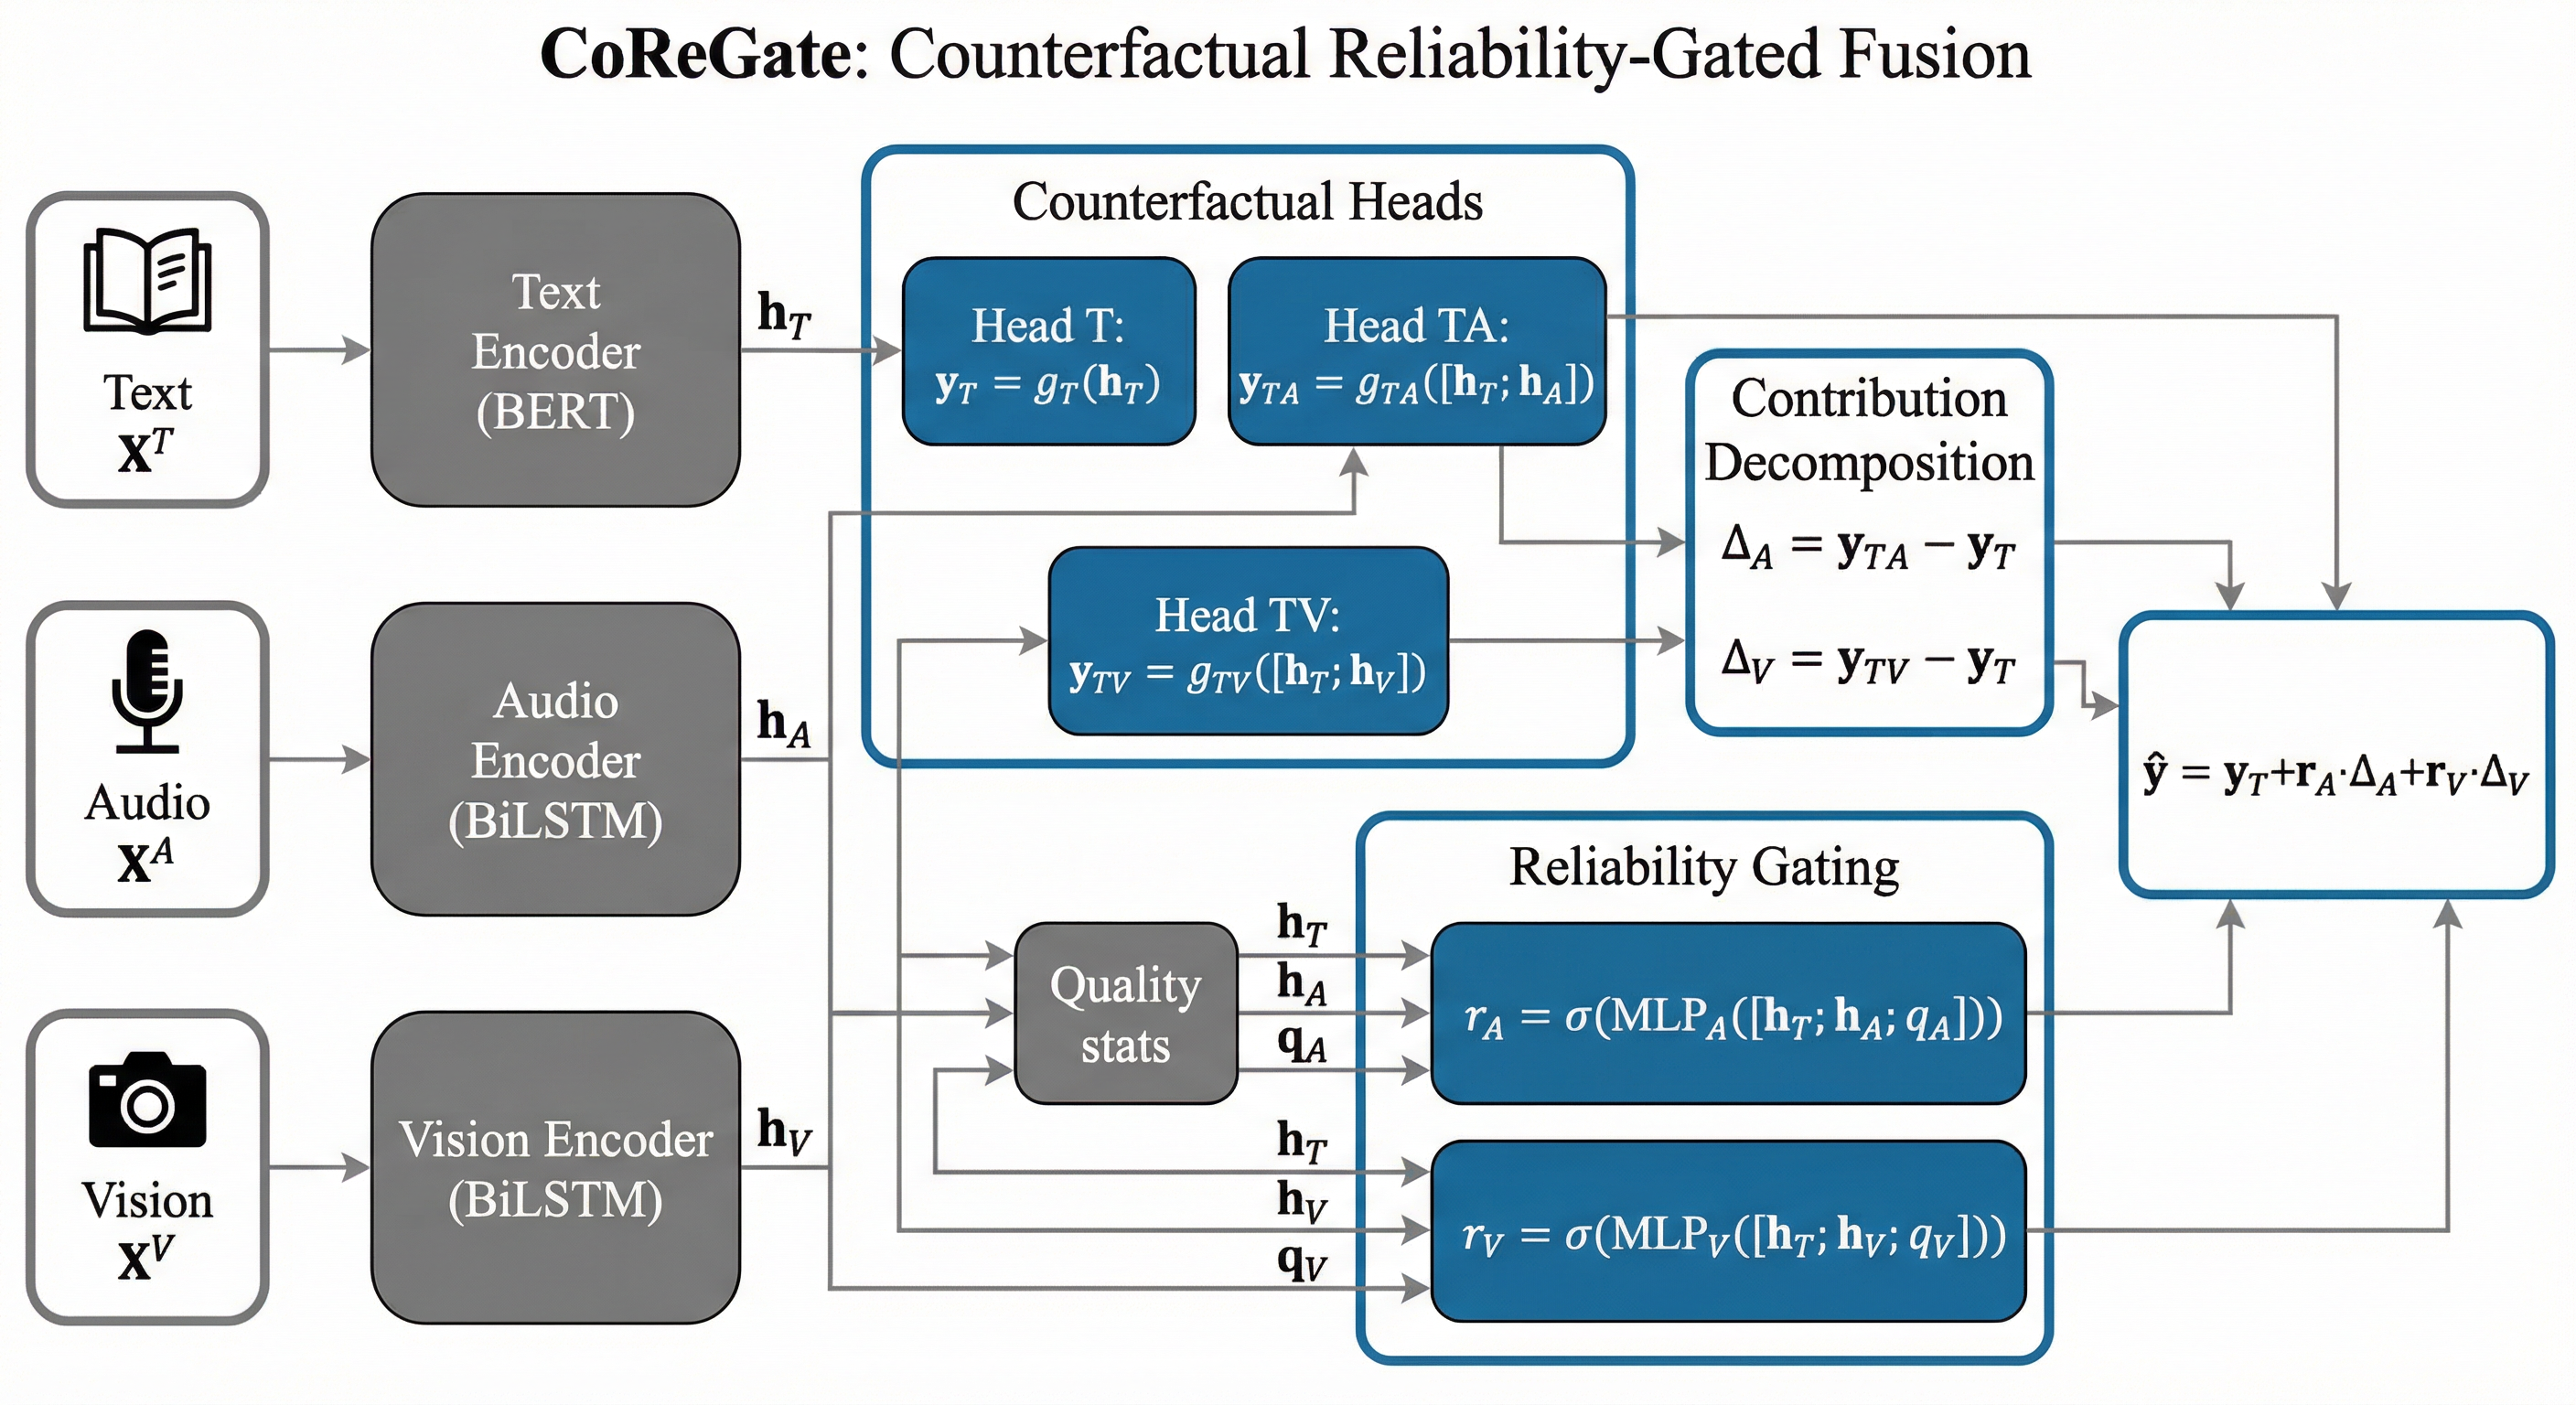
\includegraphics[scale=0.5]{fig2.pdf}
  \caption{Visualization of pseudo-label grouping based on classification confidence and localization accuracy.}
  \label{fig2}
\end{figure}
\begin{equation}
\begin{cases}
\mathcal{G}_1=(c_j,b_j)| c_j> \tau_{cls},l_j>\tau_{iou}   \\
\mathcal{G}_2=(c_j,b_j)| c_j> \tau_{cls},l_j\le\tau_{iou} \\
\mathcal{G}_3=(c_j,b_j)| c_j\le  \tau_{cls},l_j>\tau_{iou}\\
\mathcal{G}_4=(c_j,b_j)| c_j\le  \tau_{cls},l_j\le\tau_{iou}
\end{cases}
\end{equation}

Pseudo-labels in $\mathcal{G}_1$ are regarded as high-quality and are used to supervise both classification and regression. Pseudo-labels in $\mathcal{G}_2$ and $\mathcal{G}_3$ are treated as medium-quality and provide supervision only for classification or regression, respectively, depending on which component is reliable. Low-quality pseudo-labels in $\mathcal{G}_4$ are completely discarded to prevent noise propagation.
Instead of using fixed thresholds, FPG adopts category-aware adaptive thresholding following HSSDA~\cite{guo2022hssda}. For each object category $c \in \{\text{Car}, \text{Pedestrian},  \text{Cyclist}\}$ , a dynamically updated threshold set is maintained:
\begin{equation}
\mathcal{T}^c = \{\tau_{\text{cls,high}}^c, \tau_{\text{cls,low}}^c, 
\tau_{\text{roi,high}}^c, \tau_{\text{roi,low}}^c, 
\tau_{\text{iou,high}}^c, \tau_{\text{iou,low}}^c\}
\end{equation}
where thresholds are progressively refined based on confidence and IoU statistics from both labeled and unlabeled data, enabling robust pseudo-label grouping without manual tuning.
To further balance the influence of pseudo-labels from different groups, adaptive supervision weights are assigned according to pseudo-label reliability. For classification supervision, the weight is defined as:
\begin{equation}
\omega_{cls}^{(j)}=\frac{c_j}{\sum_{k\in \mathcal{G}_1\cup\mathcal{G}_2} c_k}.
\end{equation}
This design ensures that high-quality pseudo-labels dominate optimization, while medium-quality pseudo-labels provide auxiliary supervision. By explicitly leveraging partially correct predictions, FPG significantly improves pseudo-label utilization efficiency and enhances model robustness under limited annotations.
% \begin{table*}[htbp]
% \centering
% \small
% \setlength{\tabcolsep}{4pt}
% \renewcommand{\arraystretch}{1.15}
% \caption{Performance of car, pedestrian, and cyclist on the KITTI validation set.}
% \label{tab2}
% \begin{tabular}{lcccccccc}
% \toprule
% \multirow{2}{*}{Model} &
% \multicolumn{4}{c}{1\%} &
% \multicolumn{4}{c}{2\%} \\
% \cmidrule(lr){2-5} \cmidrule(lr){6-9}
% & Car & Ped. & Cyc. & mAP
% & Car & Ped. & Cyc. & mAP \\
% \midrule
% PV-RCNN          & 73.5 & 28.7 & 28.4 & 43.5 & 76.6 & 40.8 & 45.5 & 54.3 \\
% 3DIoUMatch       & 76.0 & 31.7 & 36.4 & 48.0 & 78.7 & 48.2 & 56.2 & 61.0 \\
% DDS3D            & 76.0 & 34.8 & 38.5 & 49.8 & 78.9 & 49.4 & 53.9 & 60.7 \\
% Reliable Student & 77.0 & 41.9 & 36.4 & 51.7 & 79.5 & 53.0 & 59.0 & 63.8 \\
% HSSDA            & 80.0 & 42.2 & 63.1 & 61.8 & 82.4 & 55.4 & 67.8 & 68.5 \\
% Ours             & 79.7 & 48.6 & 68.9 & 65.7 & 82.7 & 56.7 & 71.3 & 70.2 \\
% \bottomrule
% \end{tabular}
% \end{table*}
\begin{table}[htbp]
\centering
\small
\setlength{\tabcolsep}{3pt}  % 稍微减少列间距
\renewcommand{\arraystretch}{1.1}
\caption{Performance of car, pedestrian, and cyclist on the KITTI validation set.}
\label{tab2}
\resizebox{\columnwidth}{!}{  % 缩放表格到栏宽
\begin{tabular}{lcccccccc}
\toprule
\multirow{2}{*}{Model} &
\multicolumn{4}{c}{1\%} &
\multicolumn{4}{c}{2\%} \\
\cmidrule(lr){2-5} \cmidrule(lr){6-9}
& Car & Ped. & Cyc. & mAP
& Car & Ped. & Cyc. & mAP \\
\midrule
PV-RCNN          & 73.5 & 28.7 & 28.4 & 43.5 & 76.6 & 40.8 & 45.5 & 54.3 \\
3DIoUMatch       & 76.0 & 31.7 & 36.4 & 48.0 & 78.7 & 48.2 & 56.2 & 61.0 \\
DDS3D            & 76.0 & 34.8 & 38.5 & 49.8 & 78.9 & 49.4 & 53.9 & 60.7 \\
Reliable Student & 77.0 & 41.9 & 36.4 & 51.7 & 79.5 & 53.0 & 59.0 & 63.8 \\
HSSDA            & 80.0 & 42.2 & 63.1 & 61.8 & 82.4 & 55.4 & 67.8 & 68.5 \\
Ours             & 79.7 & 48.6 & 68.9 & 65.7 & 82.7 & 56.7 & 71.3 & 70.2 \\
\bottomrule
\end{tabular}
}
\end{table}
\subsection{Geometric Misalignment Overlap Upsampling}
% Point cloud sparsity and geometric misalignment significantly degrade pseudo-label reliability, especially in distant regions. To address this issue, we propose the MOU, a non-learning, geometry-aware enhancement strategy.
Point cloud sparsity and geometric misalignment not only degrade pseudo-label reliability but also create structural inconsistencies that hinder effective sensor fusion, especially in distant regions. To address this issue, we propose the MOU, a non-learning, geometry-aware enhancement strategy.

MOU selectively applies small-angle rotations to sparse regions of the point cloud and overlays the transformed points with the original input. These perturbations are restricted to low-density regions and use very small rotation angles, ensuring that global structure and local topology are preserved. Unlike conventional augmentation methods, MOU aims to compensate for geometric misalignment rather than generate artificial structures.

By enriching sparse regions with geometry-consistent overlaps, MOU provides denser and more reliable geometric cues for pseudo-label generation, improving supervision quality in the semi-supervised setting.

\subsection{Training Objective}
In the proposed semi-supervised 3D object detection algorithm, the student model is trained using both labeled and unlabeled scenes simultaneously. The overall training objective consists of the fully-supervised loss $L_l$ and semi-supervised loss $L_u$.
\begin{equation}
L_{total} = L_l + L_u 
\end{equation}
Where $L_{total}$ represents the total training loss.
For labeled scenes, we adopt the standard detection loss used in PV-RCNN \cite{31}.
% \begin{equation}
% L_l= {\textstyle \sum_{L_{cls} }(P_i^l,Y_i^l )}  +{\textstyle \sum_{L_{reg} }(P_i^l,Y_i^l)}
% \end{equation}
For unlabeled scenes and their corresponding pseudo-labels, the loss function incorporates group-specific weights to account for the varying reliability of pseudo-labels:
\begin{equation}
\begin{split}
L_u= & {\sum_{j\in \mathcal{G}_1 }(w_{cls}^{(j)}L_{cls}(P_i^u,Y_i^u)+w_{reg}^{(j)}L_{reg}(P_i^u,Y_i^u))} \\
& + \sum_{j\in \mathcal{G}_2 }(w_{cls}^{(j)}L_{cls}(P_i^u,Y_i^u)) \\
& + \sum_{j\in \mathcal{G}_3 }(w_{reg}^{(j)}L_{reg}(P_i^u,Y_i^u))
\end{split}
\end{equation}
Here, $L_{cls}$ denotes the classification loss, $L_{reg}$ denotes the bounding box regression loss, $ w_{cls}$ and $w_{reg}$ are the corresponding adaptive weights for the classification and regression loss, respectively. The student model minimizes$L_{total}$ through gradient descent, while the teacher model is updated using the EMA strategy to ensure stable and progressive improvement of pseudo-label quality.
\begin{figure}[htbp]
\centering
\includegraphics[scale=0.4]{fig3.pdf}
\caption{Overview of the MOU process for sparse point cloud regions.}
\label{fig3}
\end{figure}

% \begin{table*}[htbp]
% \centering
% \small
% \setlength{\tabcolsep}{3.5pt}
% \renewcommand{\arraystretch}{1.15}
% \caption{Performance of car, pedestrian, and cyclist on the DAIR-V2X validation set.}
% \label{tab3}
% \begin{tabular}{lccccccccccc}
% \toprule
% \multirow{2}{*}{Model} &
% \multicolumn{3}{c}{Car} &
% \multicolumn{3}{c}{Ped.} &
% \multicolumn{3}{c}{Cyc.} &
% \multirow{2}{*}{mAP} \\
% \cmidrule(lr){2-4} \cmidrule(lr){5-7} \cmidrule(lr){8-10}
% & Easy & Mod. & Hard & Easy & Mod. & Hard & Easy & Mod. & Hard & \\ 
% \midrule
% PV-RCNN & 54.5 & 44.6 & 39.0 & 11.9 & 11.5 & 11.4 & 7.6 & 5.2 & 4.6 & 21.1 \\
% HSSDA   & 58.4 & 50.2 & 47.6 & 32.3 & 32.0 & 31.2 & 21.8 & 17.5 & 17.0 & 34.2 \\
% \multirow{2}{*}{Ours} 
%         & 60.2 & 53.0 & 50.4 & 33.3 & 34.2 & 32.9 & 26.1 & 21.2 & 20.0 & 36.8 \\
%         & +1.8 & +2.8 & +3.0 & +1.0 & +2.2 & +1.7 & +4.3 & +3.7 & +3.0 & +2.6 \\
% \bottomrule
% \end{tabular}
% \end{table*}

\begin{table}[htbp]
\centering
\footnotesize  % 使用更小字体
\setlength{\tabcolsep}{2pt}
\renewcommand{\arraystretch}{1.1}
\caption{Performance of car, pedestrian, and cyclist on the DAIR-V2X validation set.}
\label{tab3}
\begin{tabular}{l@{\hspace{4pt}}cccccccccc}
\toprule
\multirow{2}{*}{Model} &
\multicolumn{3}{c}{Car} &
\multicolumn{3}{c}{Ped.} &
\multicolumn{3}{c}{Cyc.} &
\multirow{2}{*}{mAP} \\
\cmidrule(lr){2-4} \cmidrule(lr){5-7} \cmidrule(lr){8-10}
& Easy & Mod. & Hard & Easy & Mod. & Hard & Easy & Mod. & Hard & \\ 
\midrule
PV-RCNN & 54.5 & 44.6 & 39.0 & 11.9 & 11.5 & 11.4 & 7.6 & 5.2 & 4.6 & 21.1 \\
HSSDA   & 58.4 & 50.2 & 47.6 & 32.3 & 32.0 & 31.2 & 21.8 & 17.5 & 17.0 & 34.2 \\
\multirow{2}{*}{Ours} 
        & 60.2 & 53.0 & 50.4 & 33.3 & 34.2 & 32.9 & 26.1 & 21.2 & 20.0 & 36.8 \\
        & +1.8 & +2.8 & +3.0 & +1.0 & +2.2 & +1.7 & +4.3 & +3.7 & +3.0 & +2.6 \\
\bottomrule
\end{tabular}
\end{table}

\begin{table}[htbp]
\centering
\small
\setlength{\tabcolsep}{6pt}
\renewcommand{\arraystretch}{1.15}
\caption{Ablation study of our algorithm.}
\label{tab5}
\begin{tabular}{lcccccc}
\toprule
HSSDA & FPG & MOU & Car & Ped. & Cyc. & mAP \\
\midrule
\checkmark & --          & --          & 82.4 & 55.4 & 67.8 & 68.5 \\
\checkmark & \checkmark  & --          & 82.4 & 56.4 & 69.0 & 69.3 \\
\checkmark & --          & \checkmark  & 82.3 & 56.0 & 68.7 & 69.0 \\
\checkmark & \checkmark  & \checkmark  & 82.7 & 56.7 & 71.3 & 70.2 \\
\bottomrule
\end{tabular}
\end{table}
\section{Experiments}
\subsection{Datasets and settings}



% We evaluate the proposed method on two widely used benchmarks: KITTI \cite{43} and DAIR-V2X \cite{44}.
We evaluate the proposed method on two widely used benchmarks: KITTI \cite{43} and DAIR-V2X \cite{44}. Both datasets provide synchronized LiDAR point clouds and camera images, serving as standard testbeds for sensor fusion research.
Following prior semi-supervised protocols, we use 1\% and 2\% labeled data on KITTI and 2\% labeled data on DAIR-V2X. The $AP_{R40}$ metric is adopted, with IoU thresholds set to 0.7 for cars and 0.5 for pedestrians and cyclists.

Our framework is implemented on the PV-RCNN detector and trained for 80 epochs using the Adam optimizer with a batch size of 8. Standard data augmentation is applied to labeled data, while lightweight geometric perturbations are used for teacher predictions. All experiments are conducted on two NVIDIA A100 GPUs. Unless otherwise stated, the same settings are used across all experiments.


\subsection{Experiments Result}
Table 1 reports the performance comparison on the KITTI validation set.
% With 2\% labeled data, our method consistently outperforms existing semi-supervised approaches. Compared to HSSDA, we achieve mAP improvements of 0.3\%, 1.3\%, and 3.5\% for cars, pedestrians, and cyclists, respectively. Notably, the largest gains are observed for cyclists, demonstrating the effectiveness of our method under sparse and challenging conditions.
With 2\% labeled data, our method consistently outperforms existing semi-supervised approaches. Compared to HSSDA, we achieve mAP improvements of 0.3\%, 1.3\%, and 3.5\% for cars, pedestrians, and cyclists, respectively. Notably, the largest gains are observed for cyclists, demonstrating the effectiveness of our method under sparse and challenging conditions. This improvement is crucial for multimodal systems, as pedestrians and cyclists are often small and sparse in LiDAR data, making them the hardest targets to align with visual features.

With 1\% labeled data, our method significantly improves detection accuracy for pedestrians and cyclists, indicating strong robustness under extremely low-label regimes.


To evaluate generalization ability, we further conduct experiments on the DAIR-V2X dataset using 2\% labeled data. As shown in Table 2, our method achieves consistent improvements across all object categories. Compared to the PV-RCNN baseline, mAP is improved by 8.4\%, 22.7\%, and 16.0\% for cars, pedestrians, and cyclists, respectively. Compared to HSSDA, our method still provides clear gains, demonstrating that the proposed framework generalizes well to different LiDAR configurations and real-world collaborative scenarios.Figure 4 presents qualitative comparisons between the baseline and our method. The baseline model often suffers from missed detections and false positives in sparse or occluded regions. Our method successfully detects challenging targets and reduces false alarms. These results indicate that the proposed framework improves both localization accuracy and robustness.

\begin{figure}[htbp]
\centering
  \includegraphics[scale=0.38]{figure4.pdf}
  \caption{Visualize Result.}
  \label{fig4}
\end{figure}

\subsection{Ablation Study}
We conduct ablation studies on KITTI (2\% labeled data) to evaluate the contribution of each component. As shown in Table 3, both FPG and MOU independently improve detection performance. FPG enhances pseudo-label utilization by exploiting partially correct predictions, while MOU enriches sparse geometric representations.

When both modules are jointly applied, the model achieves the best performance, with an overall mAP improvement of 1.7\% over the baseline. These results demonstrate that FPG and MOU are complementary and jointly contribute to more reliable semi-supervised learning.


To further analyze the effect of FPG, we evaluate pseudo-label utilization efficiency before and after applying the proposed strategy. The utilization rate increases from 10.30\% to 48.48\%, indicating that a large number of partially correct pseudo-labels are effectively exploited rather than discarded. This result validates the core motivation of FPG and explains the observed performance improvements.


\section{Conclusion}
In this paper, we propose a semi-supervised 3D object detection framework that integrates FPG and MOU. The FPG improves pseudo-label utilization by effectively exploiting partially correct predictions, rather than relying solely on high-confidence pseudo-labels. The MOU enhances sparse point cloud representation by increasing point density in low-density regions while preserving geometric consistency. Experimental results on the KITTI benchmark demonstrate the effectiveness of the proposed method under limited labeled data, achieving consistent performance improvements. By providing denser and more accurate geometric proposals, our framework serves as a robust pre-processing stage for multimodal fusion architectures.

\vfill\pagebreak

\bibliographystyle{IEEEbib}
\bibliography{strings,refs}

\end{document}
